\documentclass[a4paper,
               %boxit,
               %titlepage,   % separate title page
               %refpage      % separate references
              ]{jacow}

\makeatletter%                           % test for XeTeX where the sequence is by default eps-> pdf, jpg, png, pdf, ...
\ifboolexpr{bool{xetex}}                 % and the JACoW template provides JACpic2v3.eps and JACpic2v3.jpg which might generates errors
 {\renewcommand{\Gin@extensions}{.pdf,%
                    .png,.jpg,.bmp,.pict,.tif,.psd,.mac,.sga,.tga,.gif,%
                    .eps,.ps,%
                    }}{}
\makeatother

\ifboolexpr{bool{xetex} or bool{luatex}} % test for XeTeX/LuaTeX
 {}                                      % input encoding is utf8 by default
 {\usepackage[utf8]{inputenc}}           % switch to utf8

\usepackage[USenglish]{babel}
%\usepackage{control}
\RequirePackage{kotex}



\ifboolexpr{bool{jacowbiblatex}}%        % if BibLaTeX is used
 {%
  \addbibresource{jacow-test.bib}
  \addbibresource{biblatex-examples.bib}
 }{}

\newcommand\SEC[1]{\textbf{\uppercase{#1}}}

%%
%%   Lengths for the spaces in the title
%%   \setlength\titleblockstartskip{..}  %before title, default 3pt
%%   \setlength\titleblockmiddleskip{..} %between title + author, default 1em
%%   \setlength\titleblockendskip{..}    %afterauthor, default 1em

%\copyrightspace %default 1cm. arbitrary size with e.g. \copyrightspace[2cm]

% testing to fill the copyright space
%\usepackage{eso-pic}
%\AddToShipoutPictureFG*{\AtTextLowerLeft{\textcolor{red}{COPYRIGHTSPACE}}}

\begin{document}


%\title{Application using timing system of RAON accelerator\thanks{Work supported by ...}}
\title{특이값 분해, Singular Value Decomposition}
\author{이상일(학번, 201460437)\thanks{silee7103@ibs.re.kr}\\
       }
\maketitle

%
\begin{abstract}
   특이값 분해(Singular Value Decompostion, SVD)는 행렬을 특정한 구조로 분해하는 방식으로, 신호처리와 통계학 등의 분야에서 자주 사용된다. 특이값 분해는 행렬의 스페트럼 이론을 임의의 직사각행렬에 대해 일반화한 것으로 불 수 있다. 스펙트럼 이론을 이용하면,직교 정사각행렬을 고유값 기저로 하여 대각행렬로 분해 할 수 있다.\cite{SVD}
\end{abstract}


\section{정의}
실수나 복소수로 이루어진 체 K의 원소로 구성되는 m x n 행렬 M에 대하여, M은 다음과 같은 세 행렬의 곲으로 분해 할 수 있다.\\

\qquad M = U $\Sigma$ V* 
\newline

여기서 각 행렬은 다음과 같은 성질을 가진다.
\begin{Itemize}
	\item U는 m x m 크기를 가지는 직교행렬이다.
	\item $\Sigma$ 는 m x n 크기를 가지며, 대각선상에 있는 원소의 값은 음수가 아니며, 나머지 원소의 값이 모두 0인 대각행렬이다.
	\item V*는 V의 켤레전치 행렬로, n x n 유티터리 행렬이다.
\end{Itemize}
행렬 M을 이와 같은 세 행렬의 곱으로 나타내는 것을 M의 특이값 분해라고 한다.
일반적으로  $\Sigma$ 행렬은 더 큰 값이 먼저 나오도록, 즉 아래의 식과 같이 구성되도록 하여 이럴 경우 $\Sigma$는 M에 따라 유일하게 결정된다.

\begin {equation}
\left(\displaystyle\sum\right)_{i,i} \ge \left(\displaystyle\sum\right)_{i+1,i+1}
\end {equation}

\section{예제}
다음과 같은 행렬 A가 있을 때, \\
 A = $
\begin{bmatrix}
1 & 0 & 0 & 0 & 2\\
0 & 0 & 3 & 0 & 0\\
0 & 0 & 0 & 0 & 0\\
0 & 4 & 0 & 0 & 0\\
\end{bmatrix}$ \\

이 행렬을 M = U $\Sigma$ V* 로 분해하면 다음과 같다.\\
 U = $
 \begin{bmatrix}
 0 & 0 & 1 & 0 \\
 0 & 1 & 0 & 0 \\
 0 & 0 & 0 & -1 \\
 1 & 0 & 0 & 0 \\
 \end{bmatrix}$, 

$\Sigma$ = $
\begin{bmatrix}
4 & 0 & 0 & 0 & 2\\
0 & 3 & 0 & 0 & 0\\
0 & 0 & \sqrt{5} & 0 & 0\\
0 & 0 & 0 & 0 & 0\\
\end{bmatrix}$, 

V* = $
\begin{bmatrix}
0 & 1 & 0 & 0 & 2\\
0 & 0 & 1 & 0 & 0\\
\sqrt{0.2} & 0 & 0 & 0 & \sqrt{0.8}\\
0 & 0 & 0 & 1 & 0\\
-\sqrt{0.8} & 0 & 0 & 0 & \sqrt{0.2}\\
\end{bmatrix}$ \\

가 되며, 여기서 특이값 분해 결과는 유일하지 않다. 예를 들어, 위의 결과에서 V*를 \\

V* = $
\begin{bmatrix}
0 & 1 & 0 & 0 & 2\\
0 & 0 & 1 & 0 & 0\\
\sqrt{0.2} & 0 & 0 & 0 & \sqrt{0.8}\\
\sqrt{0.4} & 0 & 0 & \sqrt{0.5} & -\sqrt{0.1}\\
-\sqrt{0.4} & 0 & 0 & \sqrt{0.5} & \sqrt{0.1}\\
\end{bmatrix}$ \\
 
 로 교체 할 수 있다.

\section{Other}
특이값 분해(SVD)는 고유값 분해(eigendecomposition)처럼 행렬을 대각화하는 한 방법이다. 그런데, 특이값 분해가 유용한 이유는 행렬이 정방행렬이든 아니든 관계없이 모든 m x n 행렬에 대해 적용 가능하기 때문이다. 고유값과 고유벡터 (eigenvalue \& eigenvector)에서 다루었던 고유값 분해(EVD)는 정방행렬에 대해서만 적용 가능하며 또한 정방행렬 중에서도 일부 행렬에 대해서만 적용 가능한 대각화 방법임을 상기하자. 실수공간에서 임의의 m x n 행렬에 대한 특이값분해(SVD)는 다음과 같이 정의된다

\begin{figure}[h!]
	\centering
	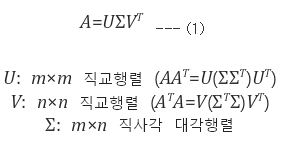
\includegraphics[width=0.4\textwidth,height=0.15\textwidth]{./svd.png}
	\caption{Singular Value Decomposition}
	\label{fig:Singular Value Decompostion} 
\end{figure}

U는 $AA^T$를 고유값분해(eigendecomposition)해서 얻어진 직교행렬(orthogonal matrix)로 U의 열벡터들을 A의 left singular vector라 부른다. 또한 V는$ A^TA$를 고유값분해해서 얻어진 직교행렬로서 V 의 열벡터들을 A의 right singular vector라 부른다.  left, right가 상당히 햇갈리는데 그냥 Σ의 왼쪽에 있는 U가 left singular 벡터, 오른쪽에 있는 V가 right 특이벡터들이라고 생각하면 된다. 마지막으로, Σ는 $AA^T$, $A^TA$를 고유값분해해서 나오는 고유값(eigenvalue)들의 square root를 대각원소로 하는 m x n 직사각 대각행렬로 그 대각원소들을 A의 특이값(singular value)이라 부른다.

\iftrue   % balancing with bad results
%	\newpage
	\raggedend
\fi

\iffalse  % only for "biblatex"
%	\newpage
	\printbibliography

% "biblatex" is not used, go the "manual" way
\else

\begin{thebibliography}{9}   % Use for  1-9  references
\bibitem{SVD}
특이값 분해 (Singular Value Decomposition, SVD):\\
%\menu[,]{for Authors,Help,Using \LaTeX}
\url{https://ko.wikipedia.org/wiki/SVD} \\

\bibitem{SVD}
[선형대수학 \#4] 특이값 분해의 활용:\\
\url{http://darkpgmr.tistory.com/106} \\



\end{thebibliography}

\fi

\end{document}
